61. \begin{figure}[ht!]
\center{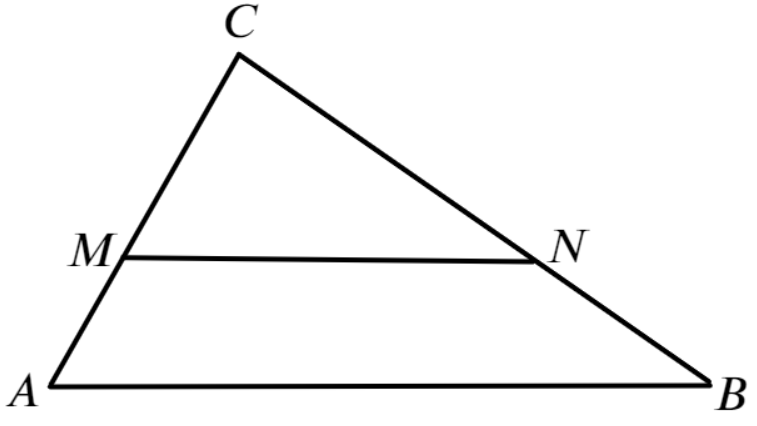
\includegraphics[scale=0.35]{g8-61.png}}
\end{figure}\\
Треугольники $MCN$ и $ABC$ подобны по двум углам (общий и соответственные при паралелльных прямых $MN$ и $AB$), коэффициент подобия равен $\cfrac{3}{3+2}=\cfrac{3}{5}.$ Тогда если $S_{\Delta ABC}=S,$ то $S_{\Delta MCN}=\cfrac{9}{25}S,$ а $S_{AMNB}=S-\cfrac{9}{25}S=\cfrac{16}{25}S,$ поэтому $\cfrac{S_{\Delta MCN}}{S_{AMNB}}=\cfrac{\cfrac{9}{25}S}{\cfrac{16}{25}S}=\cfrac{9}{16}.$\\
